
\chapter{Evaluacion}\label{capit:cap4}
\vspace{-2.0325ex}%
\noindent
\rule{\textwidth}{0.5pt}
\vspace{-5.5ex}% 
\newcommand{\pushline}{\Indp}% Indent puede ir o no :p

\section{Introducci\'on}\label{cap4:intro}
En este cap\'itulo se describe como se utilizaron los datos del experimento para lograr la detecci\'on de ansiedad. Se explica como se codificaron los eventos de ansiedad, que datos se tomaron en cuenta y los resultados de la detecci\'on por medio del uso de m\'aquinas de soporte vectorial.

\section{Codificaci\'on}
Para lograr obtener \textit{ground truth} se utilizaron varias t\'ecnicas: Observaci\'on directa, auto reportado y codificaci\'on. Se utilizaron primordialmente la observaci\'on directa y la codificaci\'on, debido a que los participantes tuvieron problemas para llenar los formatos de auto reportado en la mayor\'ia de las sesiones.

Los videos fueron primero transcritos manualmente con el programa \textit{F5 Transcription Free} para Mac OS X. Por cada video, se gener\'o un archivo en formato .txt el cual contenia el tiempo y la transcripci\'on (Ver Figura ~\ref{fig:f5transcript}). 

\begin{figure}[h]
        \centering
        \subfigure[]{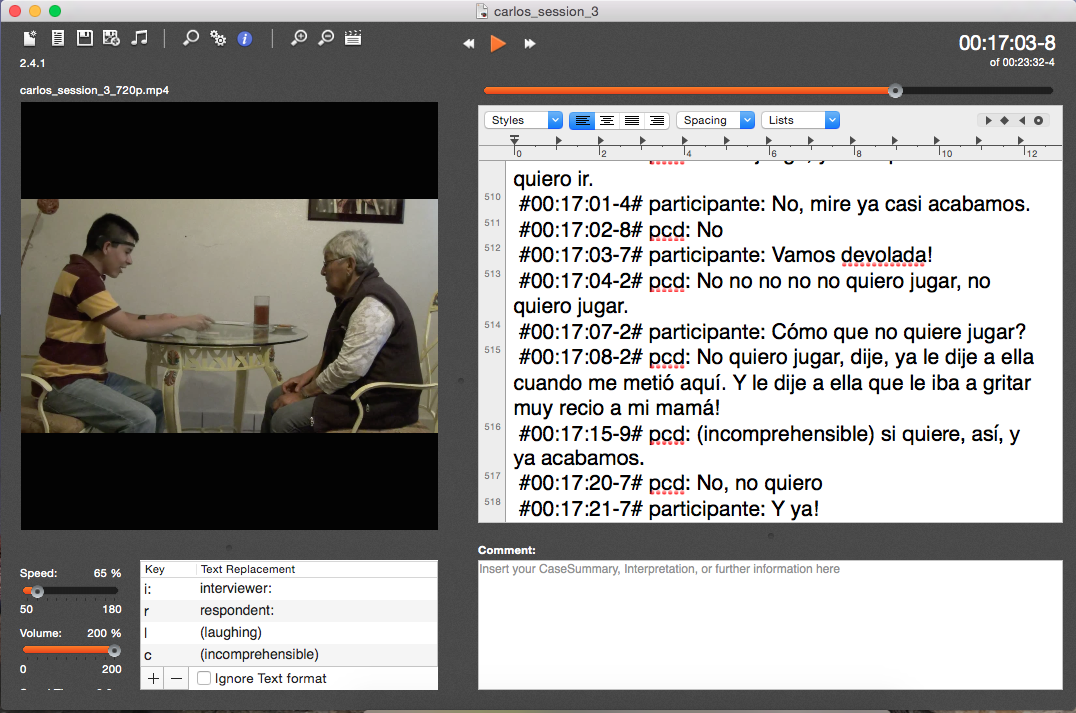
\includegraphics[height=10cm,keepaspectratio]{./Figures/img_transcript.png}}
        \caption{Transcripci\'on correspondiente a una sesi\'on completa de un participante}\label{fig:f5transcript}
\end{figure}

El archivo resultante se export\'o a Google Spreedsheets (Ver Figura: ~\ref{fig:img_codification} ) para hacer el etiquetado de segmentos de ansiedad. Esta codificaci\'on se hizo en base a la tabla de codificaci\'on (Ver tabla: ~\ref{table:anxilevels}). Se utilizaron las notas de observaci\'on recabadas para comparar que los eventos codificados a partir del video coincidieran en el tiempo y nivel de evento. Debido a que existi\'o un retraso del momento en que se inici\'o a grabar los datos fisiol\'ogicos y el momento en el que se inici\'o la grabaci\'on, se tuvieron que sincronizar los datos de la codificaci\'on. Esto se logr\'o grabando ante la c\'amara el tiempo que mostraba el tel\'efono m\'ovil encargado de la colecci\'on de los datos. Por medio de un herramienta, se sincronizaron los tiempos de la transcripci\'on en base a los segundos reportados en el video y se convirtieron de segundos a tiempo unix. La precisi\'on lograda con esta t\'ecnica fu\'e de 0 a 1 segundos.


\begin{figure}[h]
        \centering
        \subfigure[]{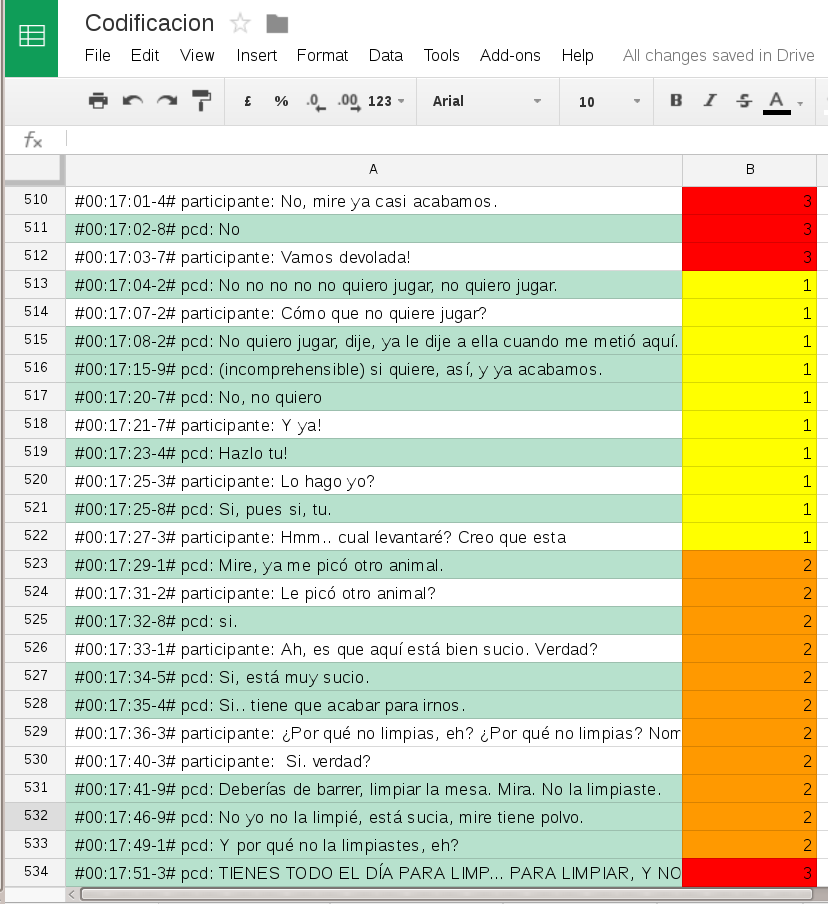
\includegraphics[height=9cm,keepaspectratio]{./Figures/img_codification.png}}
        \caption{Codificaci\'on correspondiente a una sesi\'on completa de un participante}\label{fig:img_codification}
\end{figure}

Esto permiti\'o realizar la segmentaci\'on de los eventos para su posterior an\'alisis. Tambi\'en da una visi\'on general del nivel de ansiedad observado durante toda la sesi\'on en comparaci\'on con los datos fisiol\'ogicos (Ver figura: ~\ref{fig:session_anxietylevel}).

\begin{figure}[h]
        \centering
        \subfigure[]{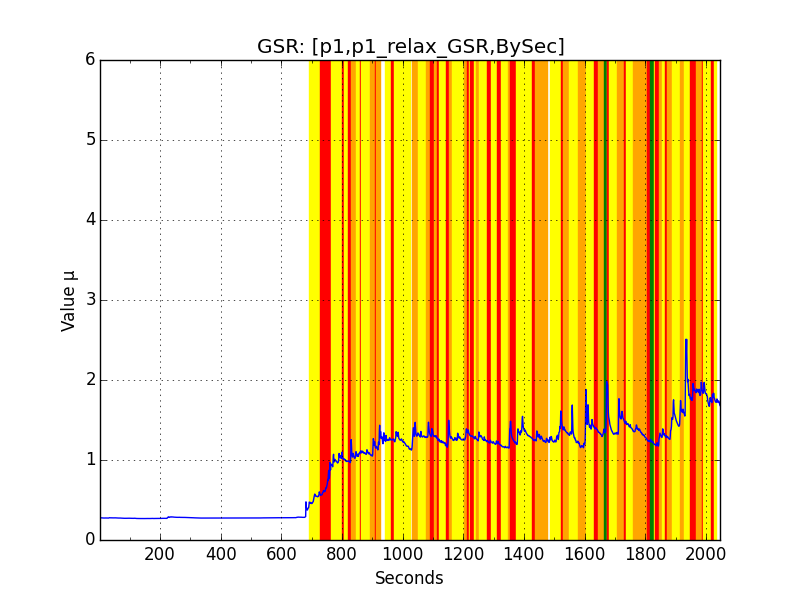
\includegraphics[height=9cm,keepaspectratio]{./Figures/img_anxietylevel.png}}
        \caption{Nivel de ansiedad observado durante una sesi\'on de un participante en comparaci\'on a su resistencia galv\'anica. Los colores indican los eventos codificados. La secci\'on grande en blanco indica el tiempo de relajaci\'on inicial.}\label{fig:session_anxietylevel}
\end{figure}

\section{Extracci\'on de caracter\'isticas}
Por cada tipo de se\~nal, se tomaron varias caracter\'isticas que generalizan un segmento de datos. La tabla ~\ref{tab:features} describe dichas caracter\'isticas.


\begin{table}[h!]
	\centering
	\caption{Caracter\'isticas usadas como entrada para el clasificador de SVM}
	\label{tab:features}
	\begin{tabular}{|l|l|l|l|l|}
		\hline
		\textbf{Se\~nal} & \textbf{Caracter\'istica} & \textbf{Descripci\'on} & \textbf{Unidad} \\
		\hline
		GSR& \pbox{12cm}{\textit{Valor en el pico}}                &  \pbox{12cm}{Valor absoluto en el pico.}             &	 \pbox{12cm}{$\mu S$} \\
		\hline
		GSR   & \pbox{12cm}{\textit{Amplitud del pico}}                & \pbox{12cm}{Distancia desde el punto\\ de crecimiento hacia el pico}             & \pbox{12cm}{$\mu S$} 	\\
		\hline
		GSR   &\textit{Valor en el punto de crecimiento}                &  \pbox{12cm}{Valor absoluto en el punto\\ de crecimiento}            &$\mu S$	 \\
		\hline
		GSR   &\textit{Indice de media recuperac\'on}                &  \pbox{12cm}{Distancia en segundos desde\\ el pico hacia el punto de \\media recuperaci\'on}            &Segundos	 \\
		\hline
		GSR   &\textit{Valor de media recuperac\'on}                &  \pbox{12cm}{Valor absoluto en el punto\\ de media recuperac\'on}	             &$\mu S$	 \\
		\hline
		GSR   &\textit{Distancia al pico anterior}                &  \pbox{12cm}{Distancia en segundos (si existe)\\ hacia el pico anterior}            &Segundos	 \\
		\hline
		HR   &\textit{M\'aximo}                & Valor m\'aximo del segmento            &BPM	 \\
		\hline
		HR   &\textit{Promedio}                & Valor promedio del segmento            &BPM	 \\
		\hline
		IBI   &\textit{M\'inimo}                & Valor m\'inimo del segmento            &Segundos	 \\
		\hline
		IBI   &\textit{Promedio}                & Valor promedio del segmento            &Segundos	 \\
		\hline
		IBI   &\textit{Desviaci\'on estandar}                &  \pbox{12cm}{Desviaci\'on estandar de todos\\ los datos del segmento}            &Segundos	 \\
		\hline
		TEMP   &\textit{M\'aximo}                & Valor m\'aximo del segmento             &$\degree C$	 \\
		\hline
		TEMP   &\textit{Promedio}                & Valor promedio del segmento            &$\degree C$ \\
		\hline

		
	\end{tabular}
\end{table}
%TODO:UPDATE THIS 
Para este trabajo, se tuvo un total de 51 segmentos del nivel 0, 177 del nivel 1, 145 del nivel 2 y 106 del nivel 3. Los datos corresponden a 5 del total de 10 de participantes. Utilizando 15 sesiones. No se procesaron todas las sesiones en su totalidad, debido al extenso tiempo necesario para transcribir los videos. Todos los segmentos fueron luego codificados en forma de vectores descriptores. Estos vectores fueron guardados en formato .csv, con la primera columna correspondiente a la etiqueta de nivel de ansiedad.

\section{Resultados de aprendizaje de m\'aquina}
Se realizaron diferentes pruebas con diferentes ``kernels'' de la m\'aquina de soporte vectorial. Se utiliz\'o el 50\% de los datos para entrenamiento y el otro 50\% para pruebas


\newpage
%%=====================================================
